\chapter{Exploratory Data Analysis with Product Classification}

\section{Item Classification and Forecasting Prioritization}
\label{subsec:item_classification_prioritization}

In addition to the ADI-CV demand classification, this work introduces an item-level categorization procedure designed to identify which products should receive greater attention during the forecasting evaluation. This distinction is relevant because not all products contribute equally to the forecasting problem. Some items present stable and representative sales behaviour, while others exhibit low volume, limited relevance, or highly idiosyncratic patterns.

The objective of this classification stage is therefore not only to describe the demand profile of each product, but also to support the selection and interpretation of the products for which forecasting accuracy is most relevant. In particular, the framework gives greater analytical attention to products classified as \textit{representative} or \textit{independent}, since these products are expected to provide more meaningful evidence regarding the effectiveness of the proposed graph-based forecasting approach.


\subsection{Complementary Item Relevance Classification}
\label{subsec:item_relevance_classification}

Although ADI-CV is useful to describe the temporal structure of demand, it does not directly indicate the relative importance of each product within the dataset. For this reason, a complementary rule-based item classification is applied. This second classification aims to distinguish products according to their sales magnitude and representativeness relative to the global item population.

Let \(S_i\) denote the total sales of item \(i\), \(M_i\) its maximum observed sales value, \(\bar{y}_i\) its mean demand, \(\sigma_i\) its standard deviation, and \(R_i\) its amplitude:

\begin{equation}
    S_i = \sum_{t=1}^{T} y_{i,t},
    \label{eq:total_sales_item}
\end{equation}

\begin{equation}
    R_i = \max_t(y_{i,t}) - \min_t(y_{i,t}).
    \label{eq:item_amplitude}
\end{equation}

The classifier is calibrated using dataset-level reference values. In the implementation, these values are derived from per-item aggregates. In particular, the tuple

\begin{equation}
    (A, B, C)
    \label{eq:abc_tuple}
\end{equation}

is used, where \(B\) represents a typical total-sales scale and \(C\) represents a typical maximum-sales scale. By default, these values are obtained from empirical quantiles of the per-item sales distribution.

The classifier also computes global reference statistics:

\begin{equation}
    (\mu^{ref}, \sigma^{ref}, R^{ref}),
    \label{eq:reference_stats}
\end{equation}

corresponding to the central tendency of item-level mean demand, standard deviation, and amplitude.

Based on these quantities, each item is assigned to one of four relevance-oriented categories:

\begin{equation}
    c_i^{rel} \in
    \{
    \text{representative},
    \text{independent},
    \text{small},
    \text{irrelevant}
    \}.
    \label{eq:relevance_classes}
\end{equation}

\paragraph{Representative items.}
An item is classified as \textit{representative} when it has sufficiently high total sales and its statistical profile is close to the global reference behaviour. More specifically, the item must satisfy a minimum sales condition:

\begin{equation}
    S_i > w_3 B,
    \label{eq:representative_sales_condition}
\end{equation}

and its mean, standard deviation, and amplitude must be mutually close relative to the reference statistics. This is evaluated through the factors:

\begin{equation}
    f_{\mu,i} = \frac{\bar{y}_i}{\mu^{ref}},
    \qquad
    f_{\sigma,i} = \frac{\sigma_i}{\sigma^{ref}},
    \qquad
    f_{R,i} = \frac{R_i}{R^{ref}}.
    \label{eq:representative_factors}
\end{equation}

The item is considered representative when:

\begin{equation}
    \frac{
        \max(f_{\mu,i}, f_{\sigma,i}, f_{R,i})
    }{
        \min(f_{\mu,i}, f_{\sigma,i}, f_{R,i})
    }
    \leq 1 + d_{max},
    \label{eq:close_factors_condition}
\end{equation}

where \(d_{max}\) controls the tolerated distance between the factors.

Representative products are particularly important for the evaluation because they reflect demand behaviour that is both relevant in magnitude and aligned with the general structure of the dataset. As a result, forecasting improvements on these products are more likely to indicate that the model captures meaningful relational and temporal patterns rather than isolated noise.

\paragraph{Irrelevant items.}
An item is classified as \textit{irrelevant} when both its total sales and maximum observed sales are low relative to the reference scales:

\begin{equation}
    S_i < w_1 B
    \quad \land \quad
    M_i < w_2 C.
    \label{eq:irrelevant_condition}
\end{equation}

These products have limited impact on the overall forecasting problem and may provide weak evidence for evaluating the effectiveness of graph-based relational information. Their low sales volume can also make performance metrics unstable, since small absolute deviations may correspond to large relative errors.

\paragraph{Small items.}
An item is classified as \textit{small} when its total sales fall between the lower relevance threshold and the intermediate sales threshold:

\begin{equation}
    w_1 B \leq S_i \leq w_3 B.
    \label{eq:small_condition}
\end{equation}

These products are not necessarily irrelevant, but their lower volume makes them less central to the forecasting evaluation. They may still be useful for robustness analysis, particularly when assessing whether the proposed model can handle lower-demand products.

\paragraph{Independent items.}
Items that do not satisfy the criteria for representative, irrelevant, or small categories are classified as \textit{independent}:

\begin{equation}
    c_i^{rel} =
    \text{independent}.
    \label{eq:independent_condition}
\end{equation}

This category captures products with sufficient relevance but whose statistical behaviour is not close enough to the global reference profile to be considered representative. These items are important because they may correspond to products with more specific, distinctive, or idiosyncratic demand dynamics. In the context of this dissertation, independent products are especially relevant because they allow the evaluation of whether graph-based neighbourhood information can improve forecasts even when the target product does not simply follow the general behaviour of the dataset.

\subsection{Dataset Classification by Product Relevance}
\label{subsec:dataset_product_classification}

In addition to the demand-pattern characterization based on ADI--CV\(^2\), the dataset was also classified according to the practical relevance and behavioural role of each product in the forecasting task. This classification is used to distinguish products that should receive greater attention during model evaluation from products whose demand is either too small or less informative for assessing relational forecasting methods.

The products are divided into three categories: \textit{representative}, \textit{independent}, and \textit{small}. Representative products correspond to items whose demand behaviour is sufficiently informative and relevant to characterize the broader dataset. These products usually have enough sales activity to support reliable model training and evaluation, and they are therefore the main focus when assessing whether the forecasting models capture meaningful demand dynamics.

Independent products are also relevant for forecasting, but their behaviour is comparatively more idiosyncratic. These series may contain demand spikes, irregular movements, or weaker alignment with the most common catalogue-level patterns. They are important because they test whether the model can forecast products whose demand evolution is less representative of the general population.

Small products correspond to low-volume items. These series typically contain many low or zero-demand observations and have a smaller operational impact when compared with the other groups. Although they remain part of the dataset, their forecasts are less central to the comparative evaluation because small absolute errors may dominate their interpretation and because their demand signal is often weaker.

The resulting classification distribution is shown below:

\begin{table}[H]
\centering
\caption{Distribution of products by classification category.}
\label{tab:product_classification_distribution}
\begin{tabular}{lrr}
\hline
\textbf{Category} & \textbf{Number of items} & \textbf{Percentage} \\
\hline
Representative & 1005 & 70.4\% \\
Independent & 318 & 22.3\% \\
Small & 104 & 7.3\% \\
\hline
Total & 1427 & 100.0\% \\
\hline
\end{tabular}
\end{table}

The majority of the catalogue is classified as representative, accounting for 70.4\% of all items. This indicates that most products exhibit sufficient demand relevance to be used as standard forecasting cases. Independent products represent 22.3\% of the dataset and form a secondary group of particular interest, since they provide a more challenging setting for evaluating whether the models can handle product-specific behaviour. Finally, small products account for 7.3\% of the catalogue and correspond to the lowest-priority group from a forecasting evaluation perspective.

Figure~\ref{fig:product_classification_examples} illustrates one example series from each category. The independent product shows a low baseline with several irregular demand spikes, suggesting a more unstable and product-specific pattern. The representative product presents a more active demand profile, with recurring variation and higher sales volume, making it more informative for model comparison. The small product exhibits lower sales values and a more limited demand signal, which motivates its separation from the main representative group.

\begin{figure}[H]
    \centering
    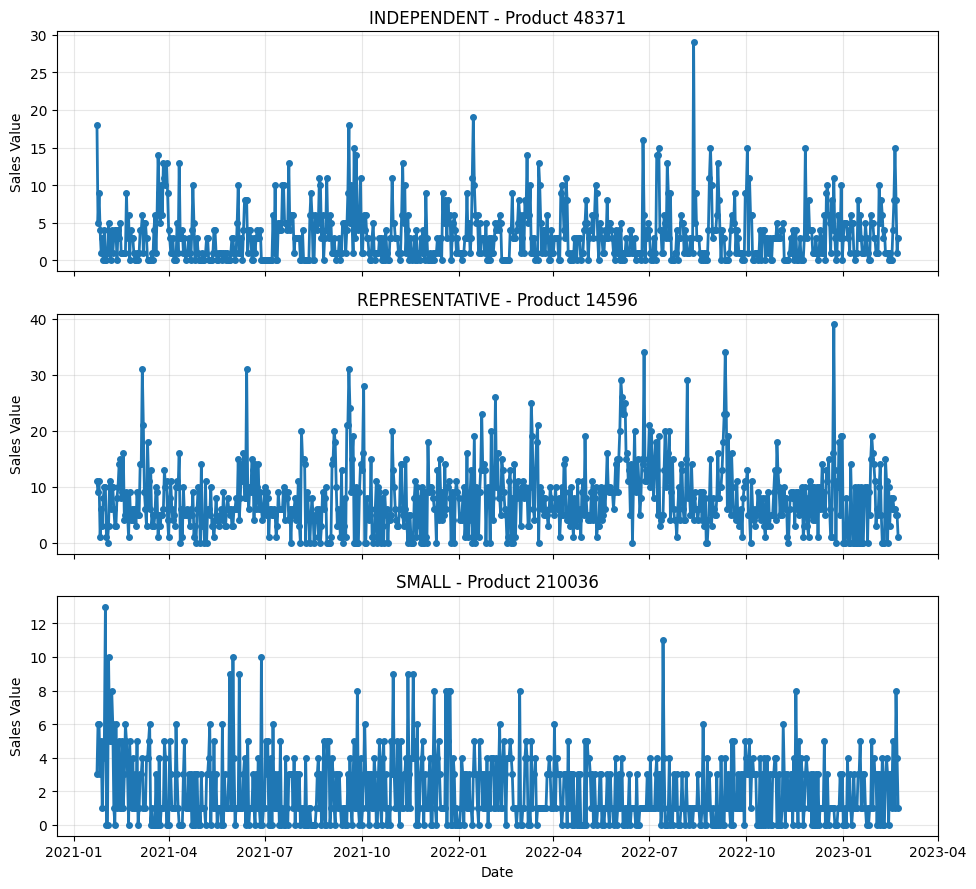
\includegraphics[width=\textwidth]{figures/representative_small_independent}
    \caption{Examples of product time series for the independent, representative, and small classification categories.}
    \label{fig:product_classification_examples}
\end{figure}

This classification is useful for interpreting the experimental results. Forecasting errors on representative products provide evidence about the model's behaviour on the most relevant portion of the catalogue, while independent products test robustness to less typical demand patterns. Small products, although included in the broader dataset description, should be interpreted with caution because their low demand volume may make error metrics less stable and less operationally meaningful.

In the initial experimental stage, the analysis focuses only on the \textit{representative} items. This choice is motivated by two main reasons. First, representative products have a sufficiently significant sales volume throughout the year, which makes their demand series more informative for training and evaluating forecasting models. Since these products exhibit enough historical activity, the resulting error metrics are less dominated by sparse or near-zero observations and provide a more reliable comparison between methods. Second, this group already accounts for a substantial portion of the catalogue, representing 1005 out of 1427 items, or 70.4\% of the dataset. Therefore, restricting the first set of experiments to representative items allows the evaluation to focus on the most operationally relevant and statistically informative part of the dataset, while still covering the majority of available products.

The independent and small categories are retained for later analysis, but the representative group is used as the primary benchmark subset in the first stage of experimentation.